%Dokumentklasse

%draft als optionohne bilder für bessere performance
%\documentclass[a4paper,12pt,]{scrreprt}

%normal mit Bildern
\documentclass[
a4paper,
12pt,
draft=True]
{scrartcl}

%Section als Chapter
\RedeclareSectionCommand[%
%beforeskip = -1sp plus -1sp minus -1sp,% kleinster negativer Wert, um den Absatzeinzug nach der Überschrift zu verhindern.
afterskip = 1.5 \baselineskip plus -1sp minus 1sp,
font = \Huge,
]{section}

\usepackage[left= 3cm,right = 3cm, bottom = 3cm,top = 3cm]{geometry}
%\usepackage[onehalfspacing]{setspace}

% ============= Packages =============
% Dokumentinformationen
\usepackage[
pdftitle={Praktikum - Umwelttechnik},
pdfsubject={},
pdfauthor={Roman-Luca Zank},
pdfkeywords={},	
%Links nicht einrahmen
hidelinks
]{hyperref}

%nur Text zum prüfen des Umfangs

% Standard Packages
%\usepackage[bottom]{footmisc}
\usepackage[utf8]{inputenc}
\usepackage[ngerman]{babel}

\usepackage[T1]{fontenc}
%\usepackage{helvet}

%\renewcommand{\familydefault}{\sfdefault}

\usepackage{graphicx}
\graphicspath{{img/}}
\usepackage{mhchem}
\usepackage{fancyhdr}
\usepackage{lmodern}
\usepackage{color}
\usepackage{placeins}
\usepackage{booktabs}
\usepackage{caption}
\usepackage[list=true]{subcaption}
\usepackage{longtable}
\usepackage{tikz}
\usepackage{pgfplots}
\usepackage{lastpage}
%\usepackage{ulem}
\usepackage{mathtools}
\usepackage{adjustbox}
\usetikzlibrary{patterns}
\usepackage{pdfpages}

%Einheitenpackage
\usepackage{siunitx}  
\sisetup{	locale = DE, 
	per-mode=fraction,
	inter-unit-product=\ensuremath{\cdot},
	detect-weight = true,
	quotient-mode=fraction
}
%neue Einheiten definieren
\DeclareSIUnit\xyz{xyz}	
\DeclareSIUnit\rpm{rpm}	
\DeclareSIUnit\mws{mWS}	
\DeclareSIUnit\degrees{^\circ}	

%Automatisch cdot statt *
\DeclareMathSymbol{*}{\mathbin}{symbols}{"01}


%Tabelle
\usepackage{tabularx}
\usepackage{tabulary}

%nur letzte Zeile der Gleichung nummerieren
\makeatletter
\def\Let@{\def\\{\notag\math@cr}}
\makeatother

% zusätzliche Schriftzeichen der American Mathematical Society
\usepackage{amsfonts}
\usepackage{amsmath}

%Abkürzungsverzeichnis
\usepackage{acronym}

%kein Abstand bei neuem Kapitel vom Seitenanfang
%\vspace*{2.3\baselineskip} = ORIGINAL
%\renewcommand*{\chapterheadstartvskip}{\vspace*{.0\baselineskip}}

%nicht einrücken nach Absatz
\setlength{\parindent}{0pt}


\urlstyle{same}

% ============= Kopf- und Fußzeile =============
\pagestyle{fancy}
%
\lhead{}
\chead{}
\rhead{}%\slshape }%\leftmark}
%%
\lfoot{}
\cfoot{}
\rfoot[{\thepage\ of \pageref*{LastPage}}]{Seite \thepage\ von \pageref*{LastPage}}
%%
\renewcommand{\headrulewidth}{0pt}
\renewcommand{\footrulewidth}{0pt}
%\renewcommand{\chapterpagestyle}{fancy}

%Fußnotelinie
%\let\footnoterule

%Fußnote mit Klammer
\renewcommand*{\thefootnote}{(\arabic{footnote})}

%Abb. statt Abbildung
\addto\captionsngerman{%
	\renewcommand{\figurename}{Abb.}%
	\renewcommand{\tablename}{Tab.}%
}

% ============= Package Einstellungen & Sonstiges ============= 
%Besondere Trennungen
%\hyphenation{De-zi-mal-tren-nung}
\usepackage[none]{hyphenat}
\hyphenpenalty=5000
\tolerance=5000
\providecommand\phantomsection{}

\usepackage{mathtools}


% ============= Dokumentbeginn =============

\begin{document}
%Seiten ohne Kopf- und Fußzeile sowie Seitenzahl
\pagestyle{empty}

%\begin{center}
\begin{tabular}{p{\textwidth}}


\begin{center}

\includegraphics[scale=0.75]{logos.jpg}\\
\end{center}


\\

\begin{center}
\LARGE{\textsc{
Protokoll \\
Physikalische Chemie\\
}}
\end{center}

\\

%\begin{center}
%\large{Fakultät für Muster und Beispiele \\
%der Hochschule Musterhausen \\}
%\end{center}
%
%\\

\begin{center}
\textbf{\Large{Ebulliometrie}}
\end{center}

\begin{center}
	\large{Gruppe 2.1 (BCUC4)}
\end{center}


\\
%\begin{center}
%zur Erlangung des akademischen Grades\\
%Bachelor of Engineering
%\end{center}


%\begin{center}
%vorgelegt von
%\end{center}

\begin{center}
\Large{\textbf{Teilnehmer:}} \\ 
\end{center}
\begin{center}
\large{
	Willy Messerschmidt}
	
\end{center}


\\

\begin{center}
\begin{tabular}{lll}
\large{\textbf{Protokollführer:}} & & \large{Willy Messerschmidt} \\
&& \\
&&\\
\large{\textbf{Datum der Versuchsdurchführung:}}&& \large{28.05.2020}\\
&&\\
\large{\textbf{Abgabedatum:}}&& \large{18.06.2020}
\end{tabular}
\end{center}

\\ \\ \\ \\ \\ 
\large{Merseburg den 17.06.2020}

\end{tabular}
\end{center}


%\include{14_danksagungen}

%\include{15_zusammenfassung}

% Beendet eine Seite und erzwingt auf den nachfolgenden Seiten die Ausgabe aller Gleitobjekte (z.B. Abbildungen), die bislang definiert, aber noch nicht ausgegeben wurden. Dieser Befehl fügt, falls nötig, eine leere Seite ein, sodaß die nächste Seite nach den Gleitobjekten eine ungerade Seitennummer hat. 
\cleardoubleoddpage

% Pagestyle für Titelblatt leer
\pagestyle{empty}

%Seite zählen ab
\setcounter{page}{0}

%Titelblatt
\begin{center}
\begin{tabular}{p{\textwidth}}


\begin{center}

\includegraphics[scale=0.75]{logos.jpg}\\
\end{center}


\\

\begin{center}
\LARGE{\textsc{
Protokoll \\
Physikalische Chemie\\
}}
\end{center}

\\

%\begin{center}
%\large{Fakultät für Muster und Beispiele \\
%der Hochschule Musterhausen \\}
%\end{center}
%
%\\

\begin{center}
\textbf{\Large{Ebulliometrie}}
\end{center}

\begin{center}
	\large{Gruppe 2.1 (BCUC4)}
\end{center}


\\
%\begin{center}
%zur Erlangung des akademischen Grades\\
%Bachelor of Engineering
%\end{center}


%\begin{center}
%vorgelegt von
%\end{center}

\begin{center}
\Large{\textbf{Teilnehmer:}} \\ 
\end{center}
\begin{center}
\large{
	Willy Messerschmidt}
	
\end{center}


\\

\begin{center}
\begin{tabular}{lll}
\large{\textbf{Protokollführer:}} & & \large{Willy Messerschmidt} \\
&& \\
&&\\
\large{\textbf{Datum der Versuchsdurchführung:}}&& \large{28.05.2020}\\
&&\\
\large{\textbf{Abgabedatum:}}&& \large{18.06.2020}
\end{tabular}
\end{center}

\\ \\ \\ \\ \\ 
\large{Merseburg den 17.06.2020}

\end{tabular}
\end{center}
 %Prokolle
%\begin{center}
\begin{tabular}{p{\textwidth}}


\begin{center}

\includegraphics[scale=0.75]{img/logos.jpg}\\
\end{center}


\\

\begin{center}
\LARGE{\textsc{
Recherche \\
Rückgewinnung von Ammoniak aus Industrieabwässern\\
}}
\end{center}

%\begin{center}
%\large{Fakultät für Muster und Beispiele \\
%der Hochschule Musterhausen \\}
%\end{center}
%
%\\
 \\
 
\begin{center}
\textbf{\Large{Seminararbeit in Medienrecherche}}
\end{center}

\begin{center}
	\large{im WiSe 2019}
\end{center}
 \\
%\begin{center}
%zur Erlangung des akademischen Grades\\
%Bachelor of Engineering
%\end{center}


\begin{center}
\large{vorgelegt von}
\end{center}
\\


\begin{center}
\Large{\textbf{Roman-Luca Zank}} \\
\end{center}

\begin{center}
3. Semester \\
Chemie- und Umwelttechnik \\
\end{center}


\begin{center}
\begin{tabular}{lll}
	\textbf{E-Mail:} & & romanzank@mail.de\\
	\textbf{Matrikelnummer:} & &25240\\
	\textbf{Adresse:} & &Platz der Bausoldaten 2, Zimmer 224\\
	\textbf{Ort:} & &06217 Merseburg\\
	&& \\
	\textbf{Prüfer:} & & Dr. Frank  Baumann\\
\end{tabular}
\end{center}

\\ \\ \\ \\ \\
\large{Merseburg, \today}

\end{tabular}
\end{center}
 %Seminar-/Abschlussarbeit

% Pagestyle für Rest des Dokuments
\pagestyle{fancy}

%Inhaltsverzeichnis
\tableofcontents
\thispagestyle{empty}
\newpage

%Inhalt
%
%Verzeichnis aller Bilder
\label{sec:bilder}
\listoffigures
\addcontentsline{toc}{chapter}{Abbildungsverzeichnis}
\thispagestyle{empty}

%Verzeichnis aller Tabellen
\label{sec:tabellen}
\listoftables
\addcontentsline{toc}{chapter}{Tabellenverzeichnis}
\thispagestyle{empty}



%%Abkürzungsverzeichnis
%\setlength{\columnsep}{20pt}
%\twocolumn
%\addchap{Nomenklatur}
%\label{sec:abkurzung}
%\begin{acronym}
%\acro{kf}[$\text{k}_\text{f}$]{Durchlässigkeitsbeiwert}
%\acro{t}{Durchlaufzeit}
%\acro{tm}[$\text{t}_\text{m}$]{Mittlere Durchlaufzeit}
%\acro{V}{Volumen}
%\acro{h}{Höhe der Wassersäule}
%\acro{Q}{Volumenstrom}
%\acro{l}{Durchströmte Länge}
%\acro{A}{Grundfläche}
%\acro{d}{Durchmesser}
%
%\end{acronym}
%\subsubsection{Aufrufen einer Abkürzung}
%\acs{rT}
%\begin{verbatim}
%\acs{Abkürzung}
%\end{verbatim}

\section{Einleitung und Versuchsziel}
\label{sec:aufgabenstellung}
%In der Aufgabenstellung wird (in eigenen Worten und ganzen Sätzen) formuliert, was das Ziel des 
%Versuches ist.  
%[Beachten Sie die eigentliche Aufgabenstellung in den Versuchsanleitungen sowie die Hinweise zur Auswertung!] 

In diesem Versuch wurden Untersuchungen zum Siedeverhalten von reinem Isopropanol mit einem Ebulliometer angestellt. Ziel des Versuches ist das Erstellen einer Dampfdruckkurve und der Vergleich der erhaltenen Daten mit Werten aus der Literatur.

Das Wissen um die Dampfdrücke verschiedener Stoffe wird dringend zur Auslegung thermischer Trennverfahren wie etwa der Destillation und der Rektifikation benötigt. Aber auch bei der Nutzung des Dampf-Kraft-Prozesses und dem Umgang mit flüchtigen Chemikalien sind Dampfdruck-Temperatur-Abhängigkeiten zu beachten.
Der Dampfdruck sagt aus, bei welchem Druck sich ein Gleichgewichtszusand zwischen Flüssigkeit und Gasphase einstellt. Der Dampfdruck einer Substanz kann nur durch die Temperatur beeinflusst werden. Steigt die Temperatur, so steht den Molekülen in der Flüssigkeit mehr Energie zur Verfügung um die Phasengrenze zu überwinden. Es wechseln daher mehr Teilchen in die Gasphase und üben dann einen höheren Druck auf einander und die Gefäßwandung aus. Die Siedetemperatur beschreibt den Zustand, wenn der Dampfdruck einer Flüssigkeit den Umgebungsdruck überschreitet. Während des Siedens einer Flüssigkeit bleibt deren Temperatur konstant. Die Verdampfungsenthalpie sorgt für eine Energieabfuhr, in dem die überschüssige thermische Energie zum Wechsel des Aggregatzustandes genutzt wird. 

Zur Beschreibung des Dampfdruckes wurden im Laufe der Zeit immer neue Gleichungen entwickelt.\\
Die einfachste ist die Clapeyron-Gleichung (\ref{gl:clapeyron}). In ihr wird der Zusammenhang des Sättigungsdampfdruckes $p^\circ$ mit der Temperatur $T$ und den stoffspezifischen Konstanten $A$ und $B$ ausgedrückt. Sie gilt für jedes Phasengleichgewicht eines reinen Stoffes.

Die Clausius-Clapeyron-Gleichung \eqref{gl:CCG} wird im weiteren Verlauf unter Anderem zur Berechnung der molaren Verdampfungsenthalpie genutzt. Sie kann, wie auch die August'sche Dampfdruckgleichung \eqref{august} aus der Clapeyron-Gleichung abgeleitet werden.

Als Modell zur Beschreibung des Sättigungsdampfdruckes in Abhängigkeit wird die Antoine-Gleichung \eqref{gl:anton} genutzt. Diese basiert ebenfalls auf der Clapeyron-Gleichung. Sie ist aber besser zur Beschreibung realer Systeme geeignet, da in ihr ein dritter Stoffparameter C einbezogen wird. Die Antoine-Parameter A,B und C sind für viele Systeme bereits tabelliert. Dabei ist stets auf den temperaturabhängigen Geltungsbereich zu achten.
\begin{equation}\label{gl:clapeyron}
ln(p^\circ)=A-\frac{B}{T}
\end{equation}
\begin{flalign}\label{gl:anton}
	\lg(p)=A-\frac{B}{C+\vartheta[\si{\degreeCelsius}]}
\end{flalign}



%\section{Physikalische Hintergründe}
\label{sec:physik}

Als physikalische Hintergründe sind die folgenden Gleichungen dargestellt. Diese beschränken sich im Wesentlichen auf die \textsc{Bernoulli}-Gleichung mit deren Ableitungen, die \textsc{Reynold}szahl, sowie dem K$_V$-Wert.\\

\textsc{Bernoulli}-Gleichung:
\begin{flalign}
	p_1+z_1*g*\rho +\frac{1}{2}*\rho*(v_1)^2&= p_2+z_2*g*\rho+\frac{1}{2}*\rho*(v_2)^2
\end{flalign}

\textsc{Bernoulli}-Gleichung mit Druckverlust $\Delta p_v$:
\begin{flalign}
p_1+z_1*g*\rho +\frac{1}{2}*\rho*(v_1)^2&= p_2+z_2*g*\rho+\frac{1}{2}*\rho*(v_2)^2\boldsymbol{+\Delta p_v}
\end{flalign}

Vereinfachung mit $p_{\text{geodätisch}} = const.$ und $p_{\text{dynamisch}} = const.$:
\begin{flalign}
p_1&= p_2+\Delta p_v
\end{flalign}

Kontinuitätsgleichung:
\begin{flalign}
	\dot{V}	&= v*A\\
	\dot{V_1}&= \dot{V_2}\\
	v_1*A_1	&= v_2*A_2
\end{flalign}

Druckverluste:
\begin{flalign}
	\Delta p_v	&= \left(\lambda *\frac{l}{d}+\sum\zeta_i\right)*\frac{\rho}{2}*v^2
\end{flalign}

\textsc{Reynold}szahl:
\begin{flalign}
	Re	&= \frac{v*d*\rho}{\eta} = \frac{v*d}{\nu}
\end{flalign}

K$_V$-Wert:
\begin{flalign}
K_V	&= \dot{V}*\sqrt{\frac{\SI{1}{\bar}}{\Delta p}*\frac{\rho}{\rho_0}}
\end{flalign}

%\section{Geräte und Chemikalien}
\label{sec:geraete}

\textbf{Geräte:}
\begin{itemize}
	\item Magnetrührer mit Rührfisch
	\item Bechergläser
	\item Erlenmeyerkolben
	\item Büchnertrichter
	\item Saugflasche
	\item Filterpapier
	\item Reflektometer RQflex$^{\textsuperscript{\textregistered}}$ plus 10 von \textsc{Merck}
\end{itemize}

\vspace*{5mm}

\textbf{Proben/Chemikalien:}
\begin{itemize}
	\item destilliertes Wasser
	\item Abwasserproben 1, 2 \& 3
		\item Schnelltests von \textsc{Chemsolute$^{\textsuperscript{\textregistered}}$}:
	\begin{itemize}
		\item Phosphat Test für \SI{0}{} - \SI{500}{\milli \gram \per \liter} \ce{PO4^3-} (Art.-Nr. 29500001) 
		\item Nitrat Test für \SI{0}{} - \SI{500}{\milli \gram \per \liter} \ce{NO3-} (Art.-Nr. 29350001) 
		\item Nitrit Test für \SI{0}{} - \SI{80}{\milli \gram \per \liter} \ce{NO2-} (Art.-Nr. 29300001) 
	\end{itemize}
	\item Reflectoquanten$^{\textsuperscript{\textregistered}}$ von \textsc{Merck} für Reflektometer:
	\begin{itemize}
		\item Ammonium Test für \SI{0.2}{} - \SI{7.0}{\milli \gram \per \liter} \ce{NH4+} (Art.-Nr. 1168920001) 
		\item Phosphate Test für \SI{5}{} - \SI{120}{\milli \gram \per \liter} \ce{PO4^3-} (Art.-Nr. 1169780001) 
		\item Nitrat Test für \SI{3}{} - \SI{90.0}{\milli \gram \per \liter} \ce{NO3-} (Art.-Nr. 1169950001) 
		\item Nitrit Test für \SI{0.5}{} - \SI{25.0}{\milli \gram \per \liter} \ce{NO2-} (Art.-Nr. 1169730001) 
	\end{itemize}
\end{itemize}








\section{Versuchsdurchführung}
\label{sec:durchfuerung}

Der Versuch muss zwingend in einem Abzug durchgeführt werden, weil die verwendeten Stoffe leicht flüchtig, entflammbar und gesundheitsgefährdend sind. Die in Abb. \ref{fig:zirkulationsapparatur} dargestellte Zirkulationsapparatur wurde im ersten Teil des Versuches mit etwa \SI{65}{\milli\liter} reinem Ethanol befüllt. Es ist darauf zu achten, dass alle Hähne verschlossen sind. Die Kühlwasserzufuhr für den Kondensator wurde freigegeben und die elektrische Heizung eingeschaltet. Die an der Heizung anliegende Spannung darf die \SI{180}{\volt} nicht übersteigen. Am elektrischen Thermometer wird die Temperatur der siedenden Flüssigphase abgelesen. Vor jeder Probennahme ist auf die Ausbildung des thermischen Gleichgewichtes zu warten und die Heizung abzustellen. Die Probennahme muss anschließend zügig durchgeführt werden. Dazu wird die für diesen Zweck vorgesehene und beschriftete Spritze in den jeweiligen Siphon herab gesenkt und etwa \SI{1}{\milli\liter} der Flüssigkeit angesaugt. Dabei wird die Probe der flüssigen Phase aus dem Siphon 3 und die Probe für die kondensierte Dampfphase aus dem Siphon 4 gezogen. Anschließend ist das entfernte Volumen an Flüssigkeit durch eine entsprechende Menge der jeweils weniger enthaltenen Komponente zu ersetzen. Zu Anfang liegt reiner Ethanol vor, weswegen nach jeder Probennahme Cyclohexan zugegeben wird. Um den azeotropen Punkt zu umgehen, wird das Ethanol-Cyclohexan-Gemisch nach der 7. Messung abgelassen und durch reines Cyclohexan ersetzt. Die Zirkulationsapparatur muss gründlich mit Druckluft ausgeblasen werden um Rückstände herauszuspülen, bevor das Cyclohexan eingefüllt werden kann. Das Vorgehen ist analog zu dem beim Ethanol. Die gezogenen Proben werden mit Hilfe eines Abbe-Refraktometers auf ihren Brechungsindex untersucht. Dazu wird die Lampe des Refraktometers eingeschaltet und die Probe in das dafür vorgesehene Loch am Probenträger eingespritzt. Mit Hilfe des rechten Stellrades und dem Blick durch das rechte Okular, wird ein klarer und möglichst scharfer Horizont am Fadenkreuz eingestellt. Durch das linke Okular kann dann der Brechungsindex an der entsprechenden Skala abgelesen werden. Die Werte für den Brechungsindex von Flüssig- und Dampfphase werden zusammen mit der abgelesenen Gleichgewichtstemperatur in Tabellenform notiert. Die Rohdaten dieses Versuches sind zusammen mit den Berechnungsergebnissen auf dem Vordruck im Anhang einzusehen.
Die Abfälle sind in einen Sammelbehälter zu entsorgen. Nach Beendigung aller Messungen wird die Anlage heruntergefahren. Außerdem muss die Zirkulationsapparatur wieder entleert und ausgeblasen werden.
\subsection*{Geräte und Gemikalien}

\subsubsection*{Geräte}
\begin{itemize}
	\item Zirkulationsapparatur
	\item elektronisches Thermometer
	\item Messzylinder für \SI{100}{\milli\liter}
	\item Abbe-Refraktometer
	\item Thermostat
	\item Spritzen mit Volumina zwischen \SI{2}{\milli\liter} und \SI{10}{\milli\liter}
	\item entsprechend lange Kanülen
	\item Bechergläser
	\item Abzug
	\item Trockenturm
	\item Stelltransformator
\end{itemize}
\subsubsection*{Chemikalien}
\begin{itemize}
	\item Ethanol
	\item Cyclohexan
\end{itemize}
\begin{figure}[h!]
	\centering
	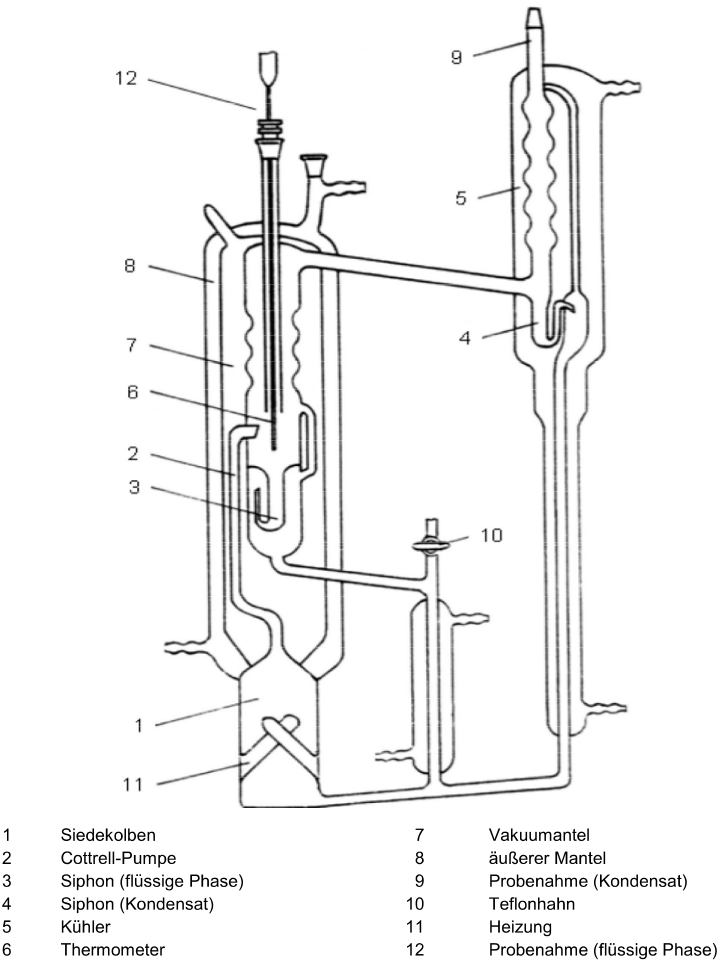
\includegraphics[width=0.7\linewidth]{img/zirkulationsapparatur}
	\caption{Beschrifteter Aufbau der Zirkulationsapparatur mit Legende}
	\label{fig:zirkulationsapparatur}
\end{figure}

\section{Ergebnisse}
\label{sec:ergebnisse}
Die Umrechnung der des gemessenen Brechungsindexes in die Anteile an Ethanol und Cyclohexan erfolgt anhand der gegeben Kalibrierung. Aus den Kalibrierdaten wird dazu eine polynomische Regressionsfunktion zweiten Grades ermittelt, anhand welcher sich durch Einsetzen der Werte für den Brechungsindex, der Anteil an Ethanol berechnen lässt. Eine Beispielrechnung dazu ist als Gleichung \eqref{gl:bsprechAnteil} nachfolgend aufgeführt. Die Berechnungsergebnisse sind in der Tabelle auf dem Vordruck eingetragen. Die Berechnung des Anteils des zweiten Stoffes Cyclohexan ist anhand der Gleichung \eqref{gl:anteilcyclo} nachzuvollziehen. 

\begin{figure}[h!]
	\begin{center}
		%\resizebox{0.8\textwidth}{!}{
		\begin{tikzpicture}[trim axis left, trim axis right]
		\begin{axis}[
		axis lines = left,
		width = 13cm,
		height = 7cm,
		xmin = 0,
		xmax = 1.05,
		ymin = 1.3,
		ymax = 1.47,
		ytick = {1.3,1.35,...,1.5},
		xtick = {0,0.1,...,1.1},
		ylabel={Brechungsindex},
		y label style={at={(-0.03,0.5)}},
		xlabel={x(Ethanol)},
		legend style={at={(0.1,0.95)},anchor=west}
		]
		\addplot table {kalibrierpunkte.dat};
		
		\addplot +[mark=none, dashed, black, domain=0:1.1] {-0.0262541672*x^2-0.0374560519*x+1.4232079871};
		\legend{Messpunkte der Kalibrierung,Kalibrierfunktion mit R$^2$=\SI{0,999}{} (\ref{gl:Regressionsgeradengleichung})};
		\end{axis}
		\end{tikzpicture}
		%	}Ventilkennlinie
		\caption{Kalibriergerade für Brechungsindex und Ethanolanteil}
		\label{dia:kalibrierung}
	\end{center}
\end{figure}
\FloatBarrier
\vspace*{-5mm}

\begin{equation}\label{gl:Regressionsgeradengleichung}
f(x)=y=-0,0262541672*x^2-0,0374560519*x+1,4232079871
\end{equation}
\begin{flalign}\label{gl:bsprechAnteil}
	x_{(\ce{EtOH})}&=-1,9045*10^{-9}*\left(	\sqrt{-1,0502*10^{19}*(\hspace{1.5mm} SW\hspace{1mm}-1,4366)}-374560519	\right)\\
	&=-1,9045*10^{-9}*\left(\sqrt{-1,0502*10^{19}*(1,361-1,4366)}-374560519\right)\\
	&=\underline{0,983}
	\end{flalign}
\begin{flalign}\label{gl:anteilcyclo}
	x_{(\ce{C6H12})}&=1-x_{(\ce{EtOH})}\\
	&=1-0,983\\
	&=\underline{0,017}
\end{flalign}


Die Berechnung der Dampfdrücke der Komponenten bei der entsprechenden Temperatur beruht auf der Antoine-Gleichung. Die benötigten Antoine-Parameter sind im Anhang der Praktikumsanleitung gegeben. Die Gleichung \eqref{gl:bspDampfdruck} enthält eine Beispielrechnung für dem Dampfdruck des Ethanols bei \SI{73,456}{\degreeCelsius}.

\begin{flalign}\label{gl:bspDampfdruck}
	lg(p^0)&=A-\frac{B}{C+\vartheta}\\
	p^0&=10^{A-\frac{B}{C+\vartheta}}\\
	&=10^{7,77534-\frac{1892,02}{249,47+\SI{73,456}{\degreeCelsius}}}\\
	&=\underline{\SI{82,480}{\kilo\pascal}}
\end{flalign}

Aktivitätskoeffizienten für die Komponenten Ethanol und Cyclohexan können über eine erweiterte Form des Raoult-Dalton'schen Gesetzes bestimmt werden. Für die Berechnung ist unter anderem auch der Umgebungsdruck wichtig. Dieser wurde am Präzisions-Quecksilberbarometer abgelesen und unter Zuhilfenahme des Programmes BARO korrigiert. Das Ergebnis für den wahren Luftdruck zu dieser Zeit im Labor lautet \SI{99,84}{\kilo\pascal}. Die Gleichung \eqref{gl:bspAktiv} enthält das entsprechende Rechenbeispiel für einen Aktivitätskoeffizienten des Ethanols.

\begin{flalign}\label{gl:bspAktiv}
	x_1^V*p&=x_1^L*p_1^0(\vartheta)*\gamma_1\\
	\gamma_1&=\frac{p*x_1^V}{p_1^0*x_1^L}\\
	&=\frac{\SI{99,84}{\kilo\pascal}*0,818}{\SI{82,480}{\kilo\pascal}*0,983}\\
	&=\underline{1,007}
\end{flalign}


Die Partialdrücke der Komponenten lassen sich vermittels des Dalton'schen Gesetzes berechnen. Eine Beispielrechnung ist dafür in Gleichung \eqref{gl:bspp1} aufgeführt. 

\begin{flalign}\label{gl:bspp1}
	p_1&=x_1^V*p\\
	&=0,818*\SI{99,84}{\kilo\pascal}\\
	&=\underline{\SI{81,675}{\kilo\pascal}}
\end{flalign}




\begin{figure}[h!]
	\centering
	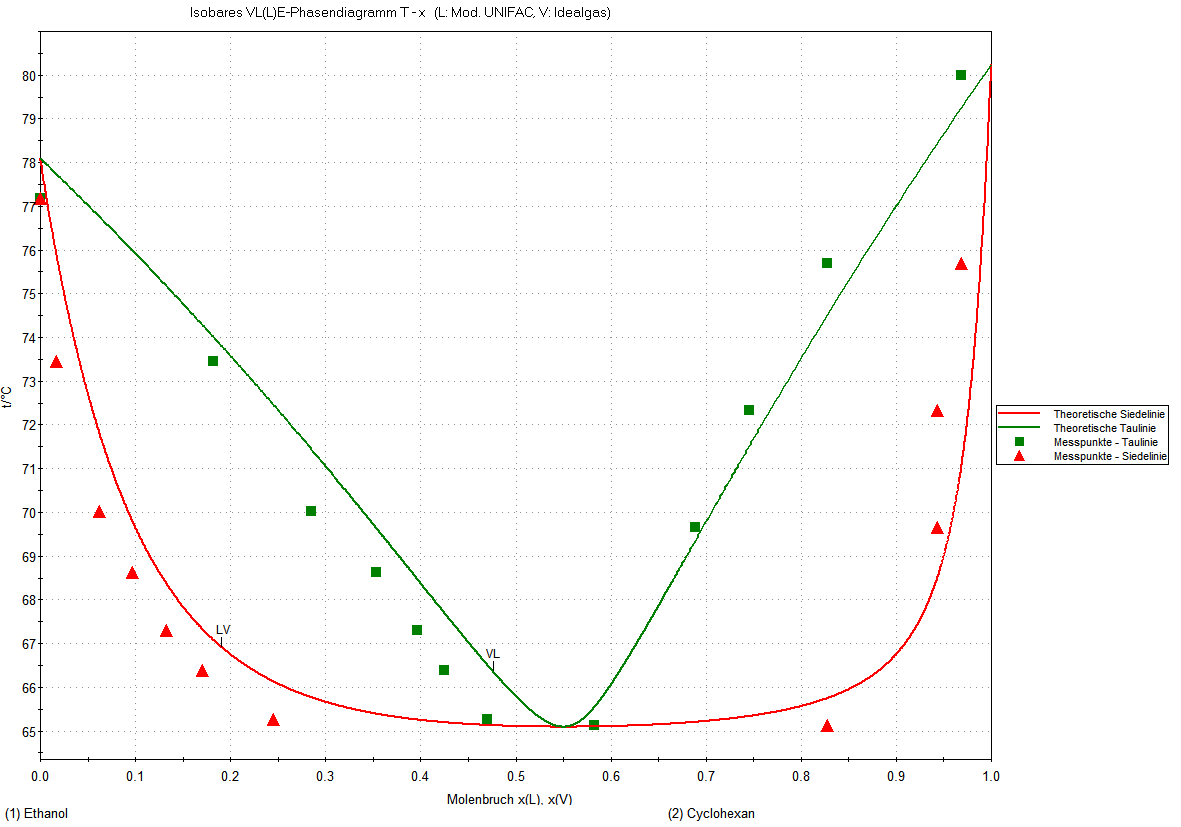
\includegraphics[width=1.1\linewidth]{img/VLE-T-x-isobar}
	\caption{Isobares Siede-/Tau-Diagramm}
	\label{fig:T-x2-isobar}
\end{figure}

\begin{figure}[h!]
	\centering
	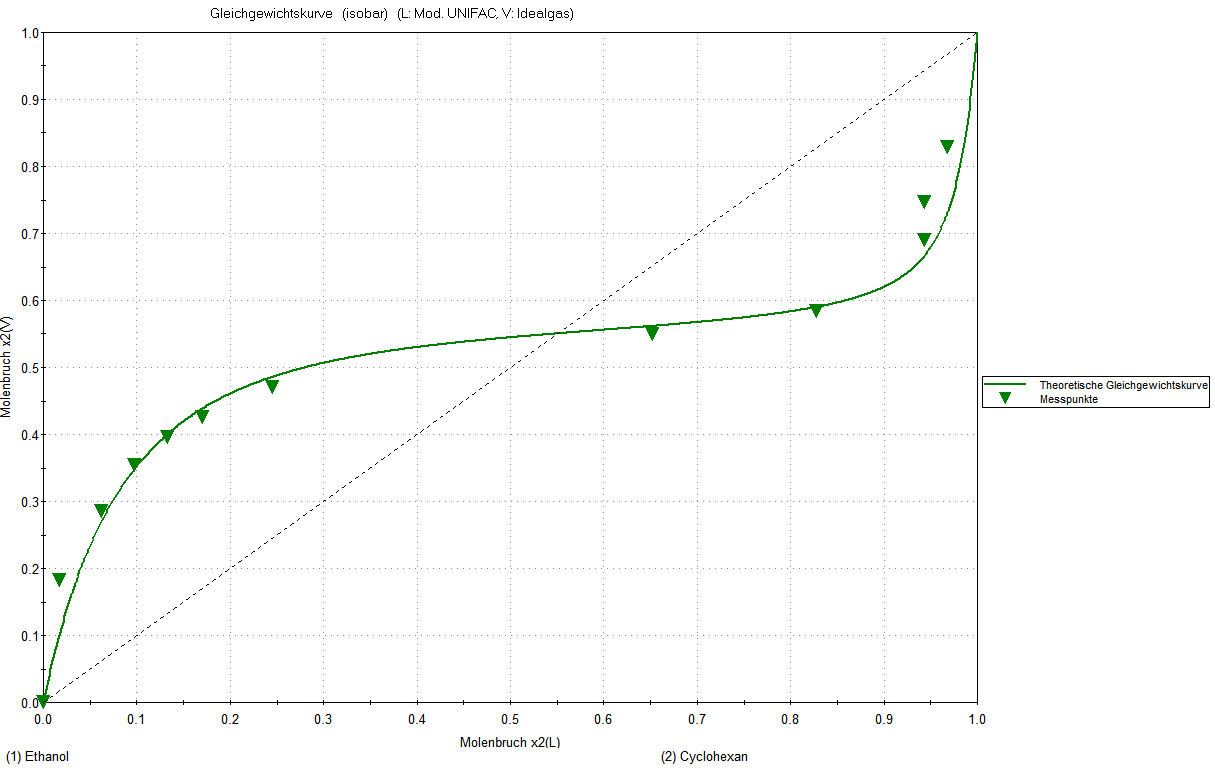
\includegraphics[width=1.1\linewidth]{img/gleichgewichtsdiagramm}
	\caption{Das Gleichgewichtsdiagramm in Anteilen von Cyclohexan}
	\label{fig:gleichgewichtsdiagramm}
\end{figure}


\begin{figure}[h!]
	\centering
	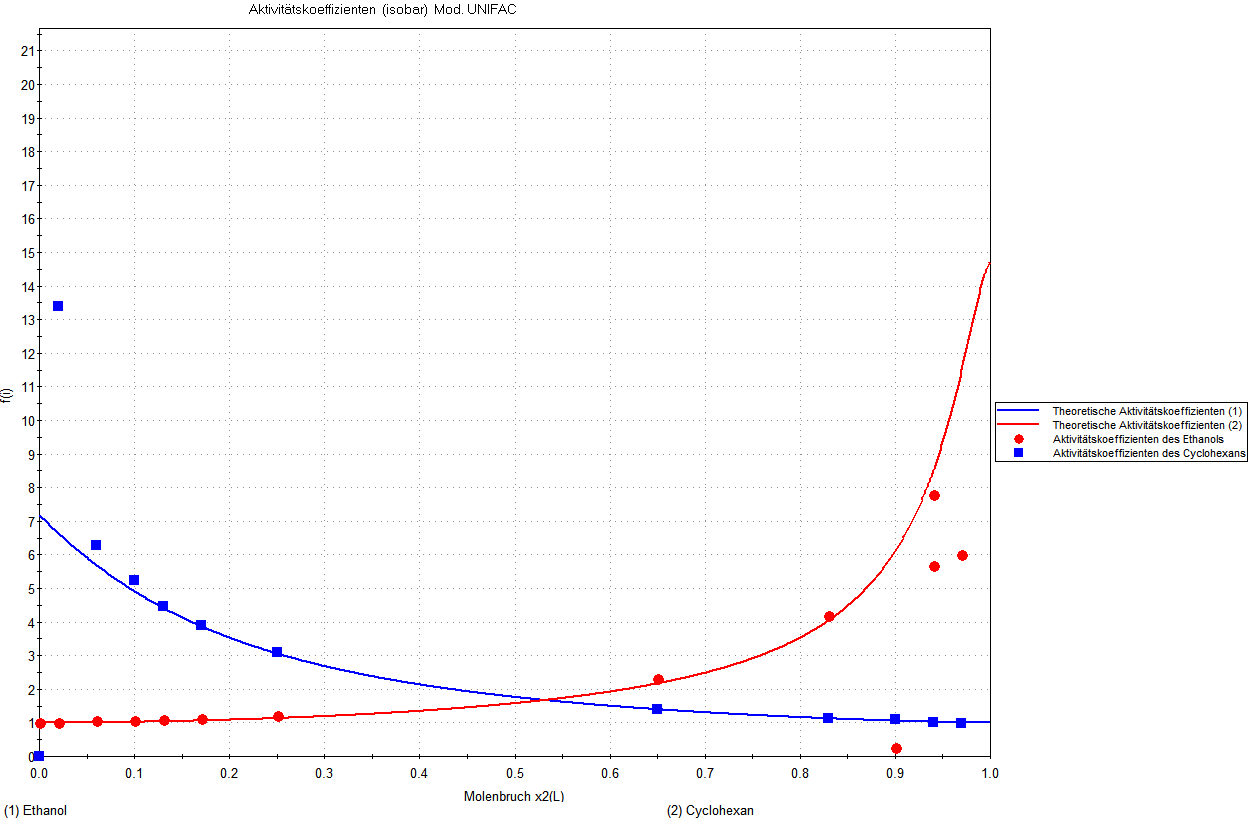
\includegraphics[width=1.1\linewidth]{img/Aktiv}
	\caption{Aktivitätskoeffizienten über dem Cyclohexananteil der flüssigen Phase}
	\label{fig:Aktiv}
\end{figure}











%%Tabelle START
%\vspace*{-5.5mm}
%\renewcommand{\arraystretch}{1.2}
%\begin{table}[h!]
%	\centering
%	\caption{Messwerttabelle und entsprechende Literaturwerte}
%	\label{tab:messwerttabelle}
%	%\resizebox{12.6cm}{!}{
%	\begin{tabular}{|c|c|c|c|}
%		\hline
%		\textbf{Nr.} &\textbf{p [\si{\kilo\pascal}]}	& \textbf{$\vartheta_{Messung}$ [\si{\degreeCelsius}]} &\textbf{$\vartheta_{Literatur}$ [\si{\degreeCelsius}] \cite{lideCRCHandbookChemistry1994}}	 \\
%		\hline
%		1& 100 & 81,4 & 82,2 \\
%		2& 90 & 78,8 & 79,8 \\
%		3& 80 & 76,0 & 77,2\\
%		4& 70 & 72,8 & 74,3\\
%		5& 60 & 69,2 & 71,1\\
%		6& 50 & 65,1 & 67,3\\
%		7& 40 & 60,3 & 62,8\\
%		8& 30 & 54,3 & 57,1\\
%		9& 25 & 50,6 &  53,4\\
%		10& 20 & 46,3 & 48,6\\
%		11& 10 & 33,7 & 24,1\\
%		\hline
%	\end{tabular}
%	%	}
%\end{table}
%\FloatBarrier
%\vspace*{-2.5mm}
%%Tabelle Ende
%
%In der Abb. \ref{dia:p/Tmess} sind die bestimmten Dampfdruckwerte als Funktion der Temperatur aufgetragen. Die Daten können der Tab. \ref{tab:messwerttabelle} entnommen werden.
%
%\begin{figure}[h!]
%	\begin{center}
%		%\resizebox{0.8\textwidth}{!}{
%		\begin{tikzpicture}[trim axis left, trim axis right]
%		\begin{axis}[
%		axis lines = left,
%		width = 13cm,
%		height = 7cm,
%		xmin = 0,
%		xmax = 110,
%		ymin = 0,
%		ymax = 110,
%		ytick = {0,10,...,100},
%		xtick = {0,10,...,100},
%		ylabel={Dampfdruck [\si{\kilo\pascal}]},
%		y label style={at={(-0.03,0.5)}},
%		xlabel={Temperatur [\si{\degreeCelsius}]},
%		legend style={at={(0.1,0.95)},anchor=west}
%		]
%		\addplot[black,mark=*,text mark as node=true,point meta=explicit symbolic,nodes near coords]
%		coordinates {(81.4, 100) (78.8, 90) (76, 80) (72.8, 70) (69.2, 60) (65.1, 50) (60.3,40) (54.3,30) (50.6,25) (46.3,20) (33.7,10)};
%		
%		\addplot +[mark=none, dashed, black, domain=1:100] {8570378.4523 * exp(-3215.05/(x + 201.633))};
%		
%		\addplot +[mark=+, black, domain=1:100] { 0.00000000425813333333321* x^5 + 0.000000773333333333376*x^4 + 0.0000366666666666613 *x^3 + 0.0032446667 *x^2 +1.11};
%		
%		\legend{{Isopropanol, experimentell},aus berechneter Antoine-Gleichung,{Isopropanol, Literatur}};
%		\end{axis}
%		\end{tikzpicture}
%		%	}Ventilkennlinie
%		\caption{Dampfdruckkurven}
%		\label{dia:p/Tmess}
%	\end{center}
%\end{figure}
%\FloatBarrier
%\vspace*{-5mm}
%Die Abb.\ref{dia:lnp/1/T} stellt die natürlichen Logarithmen der Damppfdrücke in \si{\kilo\pascal} als Funktion über der inversen Temperatur in Kelvin dar. Durch die Schaar der Messpunkte wurde durch lineare Regression im Tabellenkalkulationsprogramm \textsc{Libre-Office Calc} eine Trendlinie berechnet. Die Trendlinie geht auf die Funktionsgleichung (\ref{gl:Regressionsgeradengleichung}) zurück und besitzt ein Bestimmtheitsmaß von 0.99985.
%
%
%
%\subsection{Berechnung der molaren Verdampfungsenthalpie}\label{sec:berechnungMolareVerdEnthalpie}
%Die Berechnungs der molaren Verdampfungsenthalpie $\Delta_{LV}H_m$ baut auf der Clausius-Clapeyron-Gleichung auf. Es müssten folgende Annahmen getroffen werden.
%\begin{itemize}
%	\item Das molare Volumen der flüssigen Phase wird gegenüber dem molaren Volumen der Gasphase vernachlässigt.
%	\item Für den Dampf wird ideales Gasverhalten angenommen.
%\end{itemize}
%Daraus ergibt sich dann die Gleichung (\ref{gl:verdampfungsenthalpie}). Der linke Teil der Gleichung beschreibt dabei den Anstieg der zuvor ermittelten Regressionsgerade. Die Annahme idealen Gasverhaltens erlaubt auch die Verwendung der idealen Gaskonstante $R$.	\cite{molareVerdampfungsenthalpie}
%
%\begin{flalign}\label{gl:verdampfungsenthalpie}
%	\frac{d(\ln(p))}{d(1/T)}&=-\frac{\Delta_{LV}H_m}{R}\\
%	\SI{-5236,472}{\kelvin}&=-\frac{\Delta_{LV}H_m}{\SI{8,314}{\joule\per\mole\per\kelvin}}\\
%	\Delta_{LV}H_m&=\underline{\underline{\SI{43,536}{\kilo\joule\per\mole}}}
%\end{flalign}
%
%\subsection{Berechnung der Dampfdruckkurve aus den ermittelten \textit{ANTOINE}-Konstanten}\label{sec:berechnungDampfdruckkurveausKonstanten}
%
%Die ermittelten \textit{ANTOINE}-Konstanten derl Tab.\ref{tab:AntoineKonstanten} werden in die \textit{ANTOINE}\-Gleichung eingetragen. Dieser Schritt kann anhand der Gl.(\ref{gl:antoineEingesetzt}) nachvollzogen werden.
%\begin{flalign}\label{gl:antoineEingesetzt}
%	\lg(p)&=A-\frac{B}{C+\vartheta \,[\si{\degreeCelsius}]}\\
%	\lg(p)&=6,933-\frac{1396,28}{201,633+\vartheta\, [\si{\degreeCelsius}]}\\
%	p&=8570378,452304*e^{\frac{-3215,0535}{T+201,633}}
%\end{flalign}
%Die so erhaltene Dampfdruckkurve ist in die Abb.\ref{dia:p/Tmess} eingetragen. 

\section{Fehlerbetrachtung}
\label{sec:fehler}

Aus dem Brechungsindex der ersten Probe für den reinen Ethanol ergab sich durch die Kalibrierfunktion an Anteil größer von 1,017 und damit größer als eins. Das ist unmöglich. Daher wurde für die weiteren Berechnungen der theoretisch und praktisch einzig vertretbare Wert von eins angenommen. Nur so konnten sinnvolle Ergebnisse für die weiteren Berechnungen erhalten werden. Die Korrektur ist auch dahingehend gut vertretbar, dass die Abweichung nur sehr gering war.\\


Die Temperatur Hat großen einfluss auf die vorgenommenen Messungen. Schon kleine Differenzen wirken sich merklich auf die erhaltenen Ergebnisse aus. Von Bedeutung ist dabei vor allem die Temperatur bei welcher Kalibriert wurde, die am elektrischen Thermometer in der Zirkulationsapparatur abgelesene Temperatur und die Temperatur des Abbe-Refraktometers.

Ebenso wie die Temperatur wirkt sich auch die Wartezeit zwischen den Probenahmen direkt auf die Ergebnisse aus. Je länger der Zwischenraum, desto mehr Zeit hat die Anlage für eine gute Durchmischung und die Einstellung des thermischen Gleichgewichtes zu sorgen.

Die Dosierung mit den langkanüligen Spritzen erwies sich als sehr schwierig. Dadurch sank über die Dauer des Versuches hinweg der Flüssigkeitspegel. Undichtigkeiten mögen das Übrige dazu beigetragen haben. Dies führte zum kurzzeitigen Versagen der Cotrell-Pumpe. Der Flüssigkeitspegel wurde durch Zugabe von circa \SI{4}{\milli\liter} Cyclohexan und zwei Tropfen Ethanol angehoben. 

%\vspace*{5mm}

%\subsection*{Beispielfehlerrechnung für den ersten Messwert des rauen Rohres:}
%%Tabelle START
%\vspace*{-2.5mm}
%\renewcommand{\arraystretch}{1.2}
%\begin{table}[h!]
%	\centering
%	\caption{Abweichungen und Messwerte für die Fehlerrechnung}
%	\label{tab:abweichungen_daten}
%	\makebox[\textwidth]{
%	\begin{tabulary}{1.1\textwidth}{C|CC}
%		\hline 
%		\textbf{Messgröße} &\textbf{Messwert \linebreak(1, raues Rohr)} &\textbf{Abweichung} \\ 
%		\hline 
%		Volumenstrom & \SI{958}{\liter\per\hour} &$\pm2,5\%+MW \approx \SI{6,65e-6}{\raiseto{3}\meter \per \second}$\\ 
%		Temperatur &\SI{26,5}{\celsius} &$\pm \SI{0.5}{\kelvin} $\\ 
%		Druckmessungen & \SI{0,06}{\bar} &$2* \pm \SI{2}{\milli \mws}\approx \SI{4079}{\pascal}$\\ 
%		Durchmesser	&	\SI{13,6}{\milli \meter}&$ \pm 0$\\
%		Länge	&	\SI{2,5}{\meter}&$\pm 0$ \\
%		\hline 
%	\end{tabulary}
%	}
%\end{table}
%\FloatBarrier
%\vspace*{-5mm}
%%Tabelle Ende
%\begin{flalign}
%	\Delta p_v 	&= \frac{1}{2}*\frac{l}{d}*\rho(T)*v^2\\[5pt]
%	\lambda 	&= \frac{2*\Delta p_v*d}{l*\rho(T)*v^2}\\[5pt]
%	\label{gl:lambda}
%				&= \frac{2*\Delta p_v*d}{l*\rho(T)*\left(\frac{\dot{V}}{A}\right)^2}
%\end{flalign}
%
%Im Weiteren ist die eigentliche Fehlerrechnung für den ersten Messwert, der Messreihe des rauen Rohres, von $\lambda$ über das totale Differential der Gleichung \ref{gl:lambda} aufgeführt. Wichtig ist dabei zu erwähnen, dass alle Variablen in SI-Einheiten einzusetzen sind bis auf die Temperatur, welche in $\left[\si{\celsius}\right]$ eingesetzt wird.
%
%\subsection*{Bildung der Differentiale:}
%\begin{flalign}
%\frac{\partial \lambda}{\partial \Delta p_v} &= \frac{2*d*A^2}{l*\rho(T)*\dot{V}^2} = \frac{d^5*\pi^2}{8*l*\rho(T)*\dot{V}^2}\\[2mm]
%				&= \frac{1250*d^5*\pi^2*\left[\si{\kelvin \raiseto{3} \meter}\right]}{l*(-2683*T+10038000*\left[\si{\kelvin}\right])*\dot{V}^2*\left[\si{\kg}\right]}
%\end{flalign}
%\begin{flalign}
%	\frac{\partial \lambda}{\partial \dot{V}}	&= -\frac{4*\Delta p_v*d*A^2}{l*\rho(T)*\dot{V}^3}=-\frac{\Delta p_v*d^5*\pi^2}{4*l*\rho(T)*\dot{V}^3}\\[2mm]
%					&=- \frac{2500*\Delta p_v*d^5*\pi^2*\left[\si{\kelvin \raiseto{3} \meter}\right]}{l*(-2683*T+10038000*\left[\si{\kelvin}\right])*\dot{V}^3*\left[\si{\kg}\right]}\\[6mm]
%	\frac{\partial \lambda}{\partial T}	&=  \frac{3353750*\Delta p_v*d^5*\pi^2*\left[\si{\kelvin \raiseto{3} \meter}\right]}{l*(-2683*T+10038000*\left[\si{\kelvin}\right])*\dot{V}^2*\left[\si{\kg}\right]}
%\end{flalign}
%
%%Tabelle START
%
%\vspace*{-2.5mm}
%\renewcommand{\arraystretch}{1.2}
%\begin{table}[h!]
%	\centering
%	\caption{Ergebnisse der einzelnen Differentiale für den Messwert 1 des rauen Rohres}
%	\label{tab:differentiale}
%	%\resizebox{10cm}{!}{
%	\begin{tabulary}{\textwidth}{L|CCC}
%		\hline
%		\textbf{Differenzial} & $\frac{\partial \lambda}{\partial \Delta p_v}$ & $\frac{\partial \lambda}{\partial \dot{V}}$ &$ \frac{\partial \lambda}{\partial T }$\\ 
%		\hline
%			&\SI{3,25e-6}{\meter \raiseto{2}\second\per\kg}&\SI{-146,69}{\second\per\raiseto{3}\meter}&\SI{5,25e-6}{\per\kelvin}\\
%		\hline
%	\end{tabulary}
%	%}
%\end{table}
%\FloatBarrier
%%Tabelle Ende
%
%
%\subsection*{Berechnung des absoluten Fehlers:}
%\begin{flalign}
%	\Delta \lambda	&=  \left|\frac{\partial \lambda}{\partial \Delta p_v}\right|*\Delta p + \left|\frac{\partial \lambda}{\partial \dot{V}}\right|*\Delta \dot{V} + \left|\frac{\partial \lambda}{\partial T}\right|*\Delta T\\
%					&= \left|\SI{3,25e-6}{\meter \raiseto{2}\second\per\kg}\right|*\SI{4079}{\pascal}+ \left|\SI{-146,69}{\second\per\raiseto{3}\meter}\right|\SI{6,65e-6}{\raiseto{3}\meter \per \second}\\
%					&\nonumber \quad+\left|\SI{5,25e-6}{\per\kelvin}\right|*\SI{0,5}{\kelvin}\\[2mm]
%					&= \underline{\SI{0.0142}{}}
%\end{flalign}
%
%\subsection*{Berechnung des relativen Fehlers:}
%\begin{flalign}
%	\frac{\Delta \lambda}{\lambda}	&= \frac{0,0142}{0,0182}\\
%									&\approx \underline{\underline{\SI{78}{\percent}}}
%\end{flalign}
%%Tabelle START
%	\vspace*{-10.5mm}
%	\renewcommand{\arraystretch}{1.2}
%	\begin{table}[h!]
%		\centering
%		\caption{Absolute und relative Fehler von $\lambda$}
%		\label{tab:fehler}
%		%\resizebox{12.6cm}{!}{
%		\makebox[\textwidth]{%
%		\begin{tabular}{c|c|c|c}
%			\textbf{Messpunkt}	& \textbf{Rohrleitungswiderstand} &\textbf{Absoluter Fehler} $\left[-\right]$& \textbf{Relativer Fehler} $\left[\si{\percent}\right]$\\
%			\hline
%			\multicolumn{4}{l}{raues Rohr} \\
%			\hline
%			1&0,018&0,0142&78\\
%			2&0,020&0,0070&34\\
%			3&0,019&0,0041&21\\
%			4&0,021&0,0037&18\\
%			5&0,020&0,0031&16\\
%			\hline
%			\multicolumn{4}{l}{glattes Rohr} \\
%			\hline
%			1&0,026&0,0035&22\\
%			2&0,026&0,0029&19\\
%			(3)&(0,020)&(0,0020)&(17)\\
%			4&0,025&0,0025&17\\
%			5&0,025&0,0022&15\\
%			\hline
%			\multicolumn{4}{l}{glattes, dickes Rohr} \\
%			\hline
%			1&0,031&0,211&68\\
%			2&0,029&0,0156&54\\
%			3&0,033&0,0126&38\\
%			4&0,031&0,0108&35\\
%			5&0,031&0,0089&29\\
%			\hline
%		\end{tabular}}
%	\end{table}
%	\FloatBarrier
%	\vspace*{-2.5mm}
%	%Tabelle Ende


\section{Diskussion und Fazit}
\label{sec:diskussion}
Die Untersuchungen ergaben einen engen Zusammenhang der Temperatur und der Dampfzusammensetzung mit der Zusammensetzung der flüssigen Phase. Es wurde ein Anstieg der Aktivitätskoeffizienten bei besonders niedrigen Konzentrationen verzeichnet. Das System aus Ethanol und Cyclohexan weist einen ausgeprägten Azeotropen Punkt bei einem Anteil von rund 55\% Cyclohexan und einer Temperatur von \SI{65}{\degreeCelsius} auf. Der Vergleich des Azeotropen Punktes mit Literaturwerten \cite{azeotrop1}\cite{azeotrop2}, von \SI{64,8}{\degreeCelsius} und dem Cyclohexananteil von 43\%, ergab eine große Ähnlichkeit. Die Messergebnisse decken sich größtenteils mit den prognostizierten Werten. Aufgrund der mannigfaltigen Fehlerquellen und der in den geringeren Konzentrationen vom  UNIFAC-Modell abweichenden Aktivitätskoeffizienten sind die Messdaten dennoch mit Vorsicht zu handhaben. Die Berechnung der Wilson-Parameter entfällt, da diese nicht durch das Programm VLE unterstützt werden. \\
Eine größere Datenbasis wäre der Aussagekraft des Versuches sehr zuträglich. Außerdem könnten die Messwerte noch mit anderen Modellen und Kombinationen derer mit anderen Formeln für das Verhalten der Gase verglichen werden. Eine eigene Kalibrierung der Instrumente wäre vor dem Versuch anzustreben. So ließen sich eventuelle Fehlerquellen durch übertragung fremder Daten noch etwas einschränken. 

%\subsubsection*{a{)} Warum ist für sehr genaue Messungen eine Korrektur der am Hg-Präzisionsbarometer abgelesenen Druckwerte nötig? Um welche Art von Korrekturen handelt es sich?}
%Beim Ablesen am Barometer wird die Länge einer Quecksilbersäule betrachtet. Auf die Länge dieser Säule haben neben dem Luftdruck auch noch andere Faktoren Einfluss. Eine Korrektur des Luftdruckes ist notwendig um diese Faktoren zu kompensieren und damit eine Vergleichbarkeit der Werte zu erzeugen. Die Länge der Skala und das Volumen des Quecksilbers sind Temperaturabhängig. Temperaturschwankungen führen zu Kontraktion und Expansion. Die Korrektur erfolgt durch Umrechnung auf eine Temperatur von \SI{0}{\degreeCelsius}. Die Erdbeschleunigung "`zieht"' je nach Höhe über NN und Breitengrad unterschiedlich an der Quecksilbersäule. Korrekturstandard ist daher der 45. Breitengrad auf Meereshöhe (NN). Zuletzt muss auch der konvexe Quecksilbermenikus berücksichtigt werden welcher innerhalb des Glasrohres entsteht. Die Korrektur wurde in diesem Versuch durch das Computerprogramm BARO ausgeführt. 
%\cite{Barometerkorrektur}
%
%\subsubsection*{b{)} Erläutern Sie inwiefern Verunreinigungen in der flüssigen Phase zu einer Fehlbestimmung der temperaturabhängigen Dampfdruckwerte führen können.}
%Ist die Probe durch leichtsiedende Stoffe verunreinigt, so wird ein höherer Dampfdruck gemessen. Die verunreinigende Komponente verfälscht mit ihrem höheren Dampfdruck die Messung. Ein alltägliches Beispiel für ein ähnliches System wäre Ethanol in Wasser. Eine zweite Möglichkeit wäre die Kontamination mit einem Salz. Diese hat eine Siedepunktserhöhung zur Folge.\cite{Verunreinigungen}
%
%\subsubsection*{c{)} Stellen Sie Formel und Bedeutung der Clausius-Clapeyron-Gleichung dar und zeigen Sie durch Integration wie daraus die August'sche Dampfdruckgleichung erhalten werden kann.}
%
%Die Clausius-Clapeyron-Gleichung \eqref{gl:CCG} ist ein Sonderfall der Clapeyron-Gleichung und beschreibt den allgemeinen Zusammenhang zwischen Dampfdruck und Temperatur. Sie erlaubt es den Verlauf der Phasengrenze zwischen flüssiger und gasförmiger Phase zu berechnen.
%
%Die Umformung in die August'sche Dampfdruckgleichung hat zwei Annahmen als Voraussetzung. Zum Ersten wird ideales Gasverhalten angenommen. 
%
%\begin{flalign}\label{gl:CCG}
%	\frac{dp}{dT}&=\frac{\Delta H_{m,v}}{\Delta V_{m,v}*T}
%\end{flalign}
%Zum Zweiten wird das molare Volumen der Flüssigkeit gegenüber dem molaren Volumen des Dampfes vernachlässigt \eqref{vernachlassigt}, wodurch für die Änderung des molaren Volumens das molare Volumen des Dampfes eingesetzt werden kann.\eqref{eingesetzt}
%\begin{flalign}\label{vernachlassigt}
%	\Delta V_{m,v}= \left( V_{m,v}^{Dampf} -  \underbrace{V_{m,v}^{Liquid}}_{\rightarrow\,0}\right)= V_{m,v}^{Dampf}
%\end{flalign} 
%
%\begin{flalign}\label{eingesetzt}
%	\frac{dp}{dT}&=\frac{\Delta H_{m,v}}{\Delta V_{m,v}^{Dampf}*T}
%\end{flalign}
%
%Aufgrund der Annahme des idealen Gasverhaltens, kann nun die ideale Gasgleichung nach dem Volumen umgestellt \eqref{idealesGG} und für das molare Volumen des Dampfes eingesetzt werden.\eqref{allesdrin}
%
%\begin{flalign}\label{idealesGG}
%	p*V&=n*R*T\\
%	V_{m,v}^{Dampf}=\frac{V}{n}&=\frac{R*T}{p}
%\end{flalign}
%\begin{flalign}\label{allesdrin}
%\frac{dp}{dT}&=\frac{\Delta H_{m,v}*p}{T^2*R}\\ 
%\frac{dp}{p}&=\frac{\Delta H_{m,v}}{T^2*R}*dT
%\end{flalign}
%Es folgt die Integration \eqref{int} des Ausdruckes zur August'schen Dampfgleichung \eqref{august}.
%\begin{flalign}\label{int}
%	\int\frac{dp}{p}&=\int\frac{\Delta H_{m,v}}{T^2*R}*dT
%\end{flalign}
%\begin{flalign}\label{august}
%	\ln\left( \frac{p_2}{p_1}\right)&=\frac{\Delta H_{m,v}}{R}* \left(\frac{1}{T2}-\frac{1}{T1}\right)
%\end{flalign}
%\subsubsection*{d{)} Wie können Sie graphisch prüfen, dass der Dampfdruck einer reinen Flüssigkeit unter Annahme idealen Verhaltens für die Gas- Flüssigkeitsphase eine exponentielle Temperaturabhängigkeit besitzt?}
%
%Die exponentielle Temperaturabhängigkeit kann gepfüft werden, in dem eine Exponentialfunktion für die gefundenen Messpunkte angenähert wird. Für den Dampfdruck kann dies über die \textit{ANTOINE}-Gleichung geschehen. Für den Dampfdruck des reinen Isopropanols, unter Annahme idealen Verhaltens, ist der exponentielle Zusammenhang aus der Form der entsprechend umgestellten \textit{ANTOINE}-Gleichung \ref{sec:berechnungDampfdruckkurveausKonstanten} ersichtlich. Den endgültigen Beweis erbringt ein Blick in die Abb.\ref{dia:p/Tmess}, wo bereits erwähnte Exponentialgleichung eingetragen ist. Die Druckmesspunkte liegen praktisch auf der Exponentialfunktion und belegen so die exponentielle Temperaturabhängigkeit. 
%
%
%\subsubsection*{e{)} Wofür steht am Präzisionsthermometer der Begriff Pt-100? Erläutern sie kurz das dahinterstehende Messprinzip der Temperaturbestimmung}
%
%Die Bezeichnung Pt-100 steht für einen Platinwiderstand mit \SI{100}{\ohm}. Der elektrische Widerstand eines Leiters ändert sich mit der Temperatur. Metalle, wie auch Platin eines ist, verringern ihre Leitfähigkeit mit Steigender Temperatur, wodurch sich ihr Widerstand erhöht. Durch Messung dieses Ohm'schen Widerstandes kann anhand einer Kalibrierung auf die Temperatur des Metalls geschlossen werden.\cite{Widerstandsthermometer}
%
%\subsubsection*{f{)} Stellen Sie die bestimmten Dampfdruckwerte als Funktion der Temperatur in einem Diagramm dar.}
%
%Die Darstellung ist als Abb.\ref{dia:p/Tmess} im Kapitel \ref{sec:ergebnisse} zu finden.
%
%\subsubsection*{g{)} Erstellen Sie auf Basis ihrer Daten ein zweites Diagramm, in dem der natürliche Logarithmus des Dampfdrucks gegen die inverse Temperaturaufgetragen wird. Diskutieren Sie das Ergebnis im Hinblick auf die August'sche Dampfgleichung und beurteilen Sie die Linearität mit einer geeigneten Kenngröße. Ermitteln Sie darüber hinaus aus dem Geradenanstieg die molare Verdampfungsenthalpie $\Delta_{LV}H_m$ des untersuchten Stoffes. Vergleichen Sie mit dem entsprechenden Literaturwert und diskutieren Sie mögliche Ursachen für ggf. vorhandene Abweichungen.}
%
%Die geforderte Darstellung ist im Kapitel \ref{sec:ergebnisse} als Abb. \ref{dia:lnp/1/T} zu finden. Als Kenngröße für die Linearität wurde das Bestimmtheitsmaß der Regressionsgerade durch die Punkte aus den Wertepaaren gewählt. Dieses Bestimmtheitsmaß wird vom Tabellenkalkulationsprogramm \textsc{Libre-Office Calc} mit einem Betrag von rund 0.99985 angegeben. Dieser Wert ist sehr nah an der 1, was bedeutet, dass die gefundene Regressionsgerade sehr nah an den Punkten aus den Wertepaaren liegt. Die Linearität ist als sehr hoch einzustufen. 
%
%Die Berechnung der molaren Verdampfungsenthalpie ist im Kapitel \ref{sec:berechnungMolareVerdEnthalpie} zu finden. Aus dem Geradenanstieg ergab sich dabei eine molare Verdampfungsenthalpie des Isopropanols von rund \SI{43,5}{\kilo\joule\per\mole}. In der Literatur \cite{molareVerdampfungsenthalpieLiteraturwert} findet sich im Vergleich dazu eine molare Verdampfungsenthalpie von \SI{39,85 }{\kilo\joule\per\mole}. Der im Experiment ermittelte Wert liegt ein Wenig über dem Literaturwert. Gründe dafür sind in den Annahmen zur Berechnung zu suchen. Es wurde ein reales System untersucht. Ein solches kann sich nie vollkommen ideal verhalten. Das molare Volumen der Flüssigkeit mag zwar klein sein, aber trotzdem existiert es. Bei einer jeden Messung können systematische und zufällige Fehler Einfluss auf das Ergebnis nehmen. Näheres zu den Fehlern ist im Kapitel \ref{sec:fehler} aufgeführt.
%\subsubsection*{h{)} Mit Hilfe eines Datenauswerte-Programms, wie Excel oder ZUST, ist für die gemessenen Wertepaare p$^\circ$-T eine Regressionsrechnung durchzuführen. Dabei sind die Konstanten A, B und C der \textit{ANTOINE}-Gleichung zu bestimmen und mit Literaturwerten zu Vergleichen.}
%
%Die durch das Programm \textsc{ZUST} aus den experimentellen Daten ermittelten \textit{ANTOINE}\--Konstanten sind in der Spalte "`Experimentell"' der Tab.\ref{tab:AntoineKonstanten} eingetragen. Die ebenfalls aus dem Programm ZUST entnommenen Literaturwerte sind nebenstehend in der Spalte "`Literatur"' dargestellt. Die Literaturwerte sind deutlich höher als die im Experiment ermittelten Konstanten. Diese Abweichung kann auf den unterschiedlichen Geltungsbereich zurückzuführen sein. Die Literaturwerte gelten für einen um \SI{60}{\kelvin} weiteren Temperaturbereich als die experimentell bestimmten Werte. Das ist weit mehr als das Doppelte und relativiert eine maximale Abweichung von ca. 30\%.
%
%\begin{table}[h!]
%	\centering
%	\caption{Gegenüberstellung der experimentell ermittelten \textit{ANTOINE}-Konstanten mit Literaturwerten, sowie die zugehörigen Geltungsbereiche}
%	\label{tab:AntoineKonstanten}
%	%\resizebox{12.6cm}{!}{
%	\begin{tabular}{|c|c|c|}
%		\hline
%			\textbf{Konstante} & \textbf{Experimentell} & \textbf{Literatur} \\ 
%			\hline
%			A & 6,933 & 8,003 \\ 
%			B & 1396,28 & 2010,33 \\ 
%			C & 201,633 & 252,635\\
%		\hline
%		\hline
%		T$_\text{Lo}$ [\si{\degreeCelsius}]&33,7&-25\\
%	T$_\text{Hi}$ [\si{\degreeCelsius}]	&81,4&83\\
%	\hline
%	\end{tabular}
%	%	}
%\end{table}
%\FloatBarrier
%\vspace*{-2.5mm}
%%Tabelle Ende
%\subsubsection*{i{)} Nutzen Sie ihre ermittelten \textit{ANTOINE}-Parameter, um die p$^\circ$-T-Dampfdruckkurve mit der \textit{ANTOINE}-Gleichung zu berechnen und vergleichen Sie ihre experimentellen Werte mit den berechneten Werten im Diagramm.}
%Die Dampfdruckkurve aus den berechneten \textit{ANTOINE}-Parametern ist in der Abb. \ref{dia:p/Tmess} eingetragen. Die \textit{ANTOINE}-Gelichung mit eingesetzten Parametern ist im Kapitel \ref{sec:berechnungDampfdruckkurveausKonstanten} als Gl. (\ref{gl:antoineEingesetzt}) dargestellt. Die experimentellen Werte liegen alle sehr nah an dem berechneten Graphen. Die gefundenen \textit{ANTOINE}-Parameter beschreiben den im Experiment beobachteten Zusammenhang exakt.

\section{Zusammenfassung und Fazit}
\label{sec:zusammenfassung}

%Die experimentellen Messdaten kommen sehr nah an die Literaturwerte heran, wie aus \ref{dia:p/Tmess} hervorgeht. Das Verhalten des Isopropanols kann sehr exakt durch die Antoine-Gleichung ausgedrückt werden. Teilweise waren die Literaturwerte zum Vergleich wenig geeignet. Das erschwert die Einschätzung. Die Verwendung der Computerprogramme ZUST und BARO ermöglichte sehr präzise und belastbare Berechnungen. Noch aussagekräftigere Ergebnisse hätten durch eine mehrfach wiederholte Messung erhalten werden können. Auch eine kleinere Schrittweite bei der Einstellung der Drücke wäre sinnvoll, um sich noch genauer an die Realität anzunähern. Von Extrapolationen über den untersuchten Bereich hinaus ist dringend abzuraten.

%Praktikumsskript, Modul ………, Versuch …….., Prof. Musterprof. 
%DIN 12345, Jahr der Veröffentlichung 
%Link der Internetseite, Zugriffsdatum 
%Buchtitel, Autor, Verlag, Veröffentlichungsjahr 

%Literaturverzeichnis Bücher
\bibliography{Literatur}
\bibliographystyle{unsrtdin}
\addcontentsline{toc}{section}{Literaturverzeichnis}



\section*{Anhang}
\addcontentsline{toc}{section}{Anhang}
\label{sec:anhang}

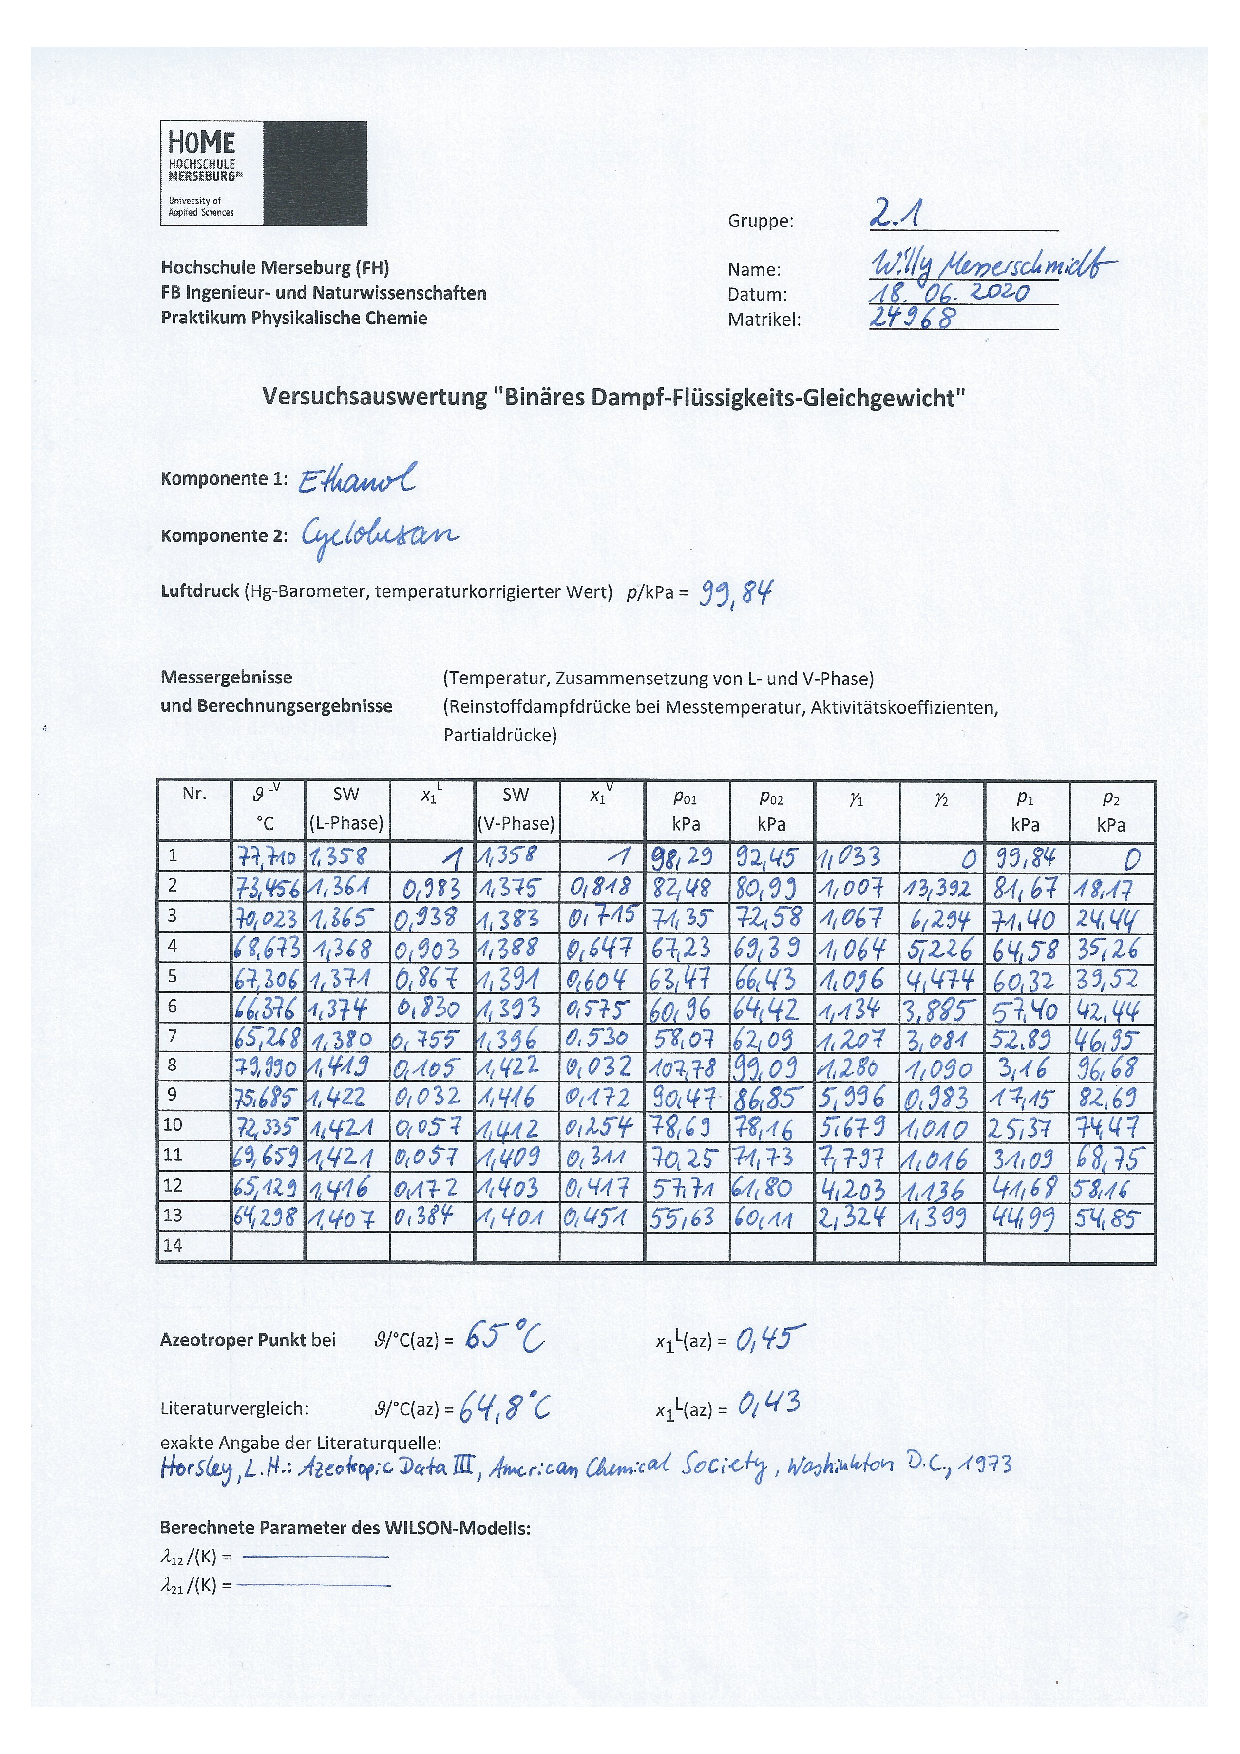
\includepdf{deckblatt}

%\chapter*{Eidesstattliche Erklärung}
\label{erklaerung}
Hiermit versichere ich, die vorliegende Seminararbeit selbstständig und nur unter Verwendung der von mir angegebenen Quellen und Hilfsmittel verfasst zu haben. Sowohl inhaltlich als auch wörtlich entnommene Inhalte wurden als solche kenntlich gemacht. Die Arbeit hat in dieser oder vergleichbarer Form noch keinem anderem Prüfungsgremium vorgelegen. \\
\\[1.5cm]
Datum:	\hrulefill\enspace Unterschrift: \hrulefill
\\[3.5cm]
\addcontentsline{toc}{chapter}{Selbstständigkeitserklärung}

\end{document}
